\documentclass[a4paper]{article}
\usepackage{geometry}
\usepackage{float}
\usepackage{longtable}
\usepackage{amsmath}
\usepackage[bottom]{footmisc}
\geometry{verbose,a4paper,tmargin=3cm,bmargin=2cm,lmargin=2cm,rmargin=3cm}
%\SweaveOpts{width=5.5, height=5.5}
\setlength{\parskip}{\medskipamount}
\setlength{\parindent}{0pt}
\usepackage{Sweave}
\begin{document}
\title{Surplus tests with MSE}
\author{Ernesto Jardim\footnote{ernesto.jardim@jrc.ec.europa.eu} (JRC)\\ Iago Mosqueira (JRC) \\ Colin Millar (JRC)\\ Chato Osio (JRC)\\ Aymen Charef (JRC)}
\maketitle
\begin{abstract}
ToDo
\end{abstract} 

\pagebreak
\section{Introduction}

The MSE runs on the ple4 dataset but it can be adapted to other datasets. The OM is conditioned using the stock assessment results and distinct S/R. The MP is based on the usual MSY HCR, with a $B_{trigger}$ and a $F_{target}$, and an additional harvest rate limit. All is dealt in relative terms. The stock status is estimated with a biomass dynamic model. The OEM introduces variability on the abundance index and bias both on the abundance index and catches. The IEM introduces bias on the catch. The bias on catch, both on the OEM and IEM must be linked so that catches on the OM are of the same level.


\begin{Schunk}
\begin{Sinput}
> sessionInfo()
\end{Sinput}
\begin{Soutput}
R version 2.15.0 (2012-03-30)
Platform: x86_64-pc-linux-gnu (64-bit)

locale:
 [1] LC_CTYPE=en_US.UTF-8       LC_NUMERIC=C              
 [3] LC_TIME=en_US.UTF-8        LC_COLLATE=en_US.UTF-8    
 [5] LC_MONETARY=en_US.UTF-8    LC_MESSAGES=en_US.UTF-8   
 [7] LC_PAPER=C                 LC_NAME=C                 
 [9] LC_ADDRESS=C               LC_TELEPHONE=C            
[11] LC_MEASUREMENT=en_US.UTF-8 LC_IDENTIFICATION=C       

attached base packages:
[1] splines   grid      stats     graphics  grDevices utils     datasets 
[8] methods   base     

other attached packages:
 [1] Hmisc_3.9-1      survival_2.36-12 xtable_1.6-0     FLBioDym_0.1.2  
 [5] FLAdvice_1.0     ggplotFL_0.1     ggplot2_0.8.9    proto_0.3-9.2   
 [9] reshape_0.8.4    plyr_1.7.1       akima_0.5-7      FLash_2.5.0     
[13] FLCore_2.5.0     lattice_0.20-6  

loaded via a namespace (and not attached):
[1] cluster_1.14.1 stats4_2.15.0  tools_2.15.0  
\end{Soutput}
\end{Schunk}

\section{Methods}

\begin{itemize}
	\item Operating Model

	$N_{t+1,a+1}=N_{t,a}e^{-Z}$
	
	$R_{t+1}=f(S_{t})\rho$ where $\rho \sim LN(0,\sigma_{R}^2)$ and $f$:{segreg,b\&h,b\&h+AR1}

	$C_{t,a}=\frac{F_{t,a}}{Z_{t,a}}(1-e^{-Z})N_{t,a}$
	
	$Y_{t}=\sum_a C_{t,a}\bar{W}_{t,a}$
	
	\item Implementation Error Model
	
	$Y_{t}=\frac{TAC_{t}}{\alpha_{t}}$

	\item Management Procedure
	
	$TAC_{t}=HCR(\hat{\Theta}_{t} | F_{trgt}, B_{trg}, HR_{max})$
	
	$\hat{\Theta}=g(\hat{C}_{t}, \hat{I}_{t})$ where $g$: biomass dynamic model 
	
	\item Observation Error Model
	
	$\hat{C}_{t}=C_{t} \alpha_{t}$ where $\alpha \sim U(0.95cthBias, 1.05cthBias)$
	
	$\hat{I}_{t} = B_{t} \gamma_{t}$ where $\gamma \sim LN(\lambda, \sigma_{I}^2)$ and $\lambda \sim U(0.95srvBias, 1.05srvBias)$	
		
\end{itemize}	

\section{Results}

\begin{table}[h]
\caption{Simulation scenarios}
% latex.default(scn, longtable = TRUE, file = "", first.hline.double = FALSE) 
%

\setlongtables


\begin{longtable}{lrrrrrr}
\hline
\multicolumn{1}{l}{scn}&\multicolumn{1}{c}{Btrig}&\multicolumn{1}{c}{CV}&\multicolumn{1}{c}{Ftar}&\multicolumn{1}{c}{aLag}&\multicolumn{1}{c}{srvBias}&\multicolumn{1}{c}{cthBias}\tabularnewline
\hline
\endhead
\hline
\endfoot
1&$0.5$&$0.2$&$1$&$1$&$1.0$&$1.0$\tabularnewline
2&$0.5$&$0.2$&$1$&$3$&$1.0$&$1.0$\tabularnewline
3&$0.5$&$0.2$&$1$&$5$&$1.0$&$1.0$\tabularnewline
4&$0.5$&$0.2$&$1$&$1$&$0.5$&$1.0$\tabularnewline
5&$0.5$&$0.2$&$1$&$3$&$0.5$&$1.0$\tabularnewline
6&$0.5$&$0.2$&$1$&$5$&$0.5$&$1.0$\tabularnewline
7&$0.5$&$0.2$&$1$&$1$&$1.0$&$0.5$\tabularnewline
8&$0.5$&$0.2$&$1$&$3$&$1.0$&$0.5$\tabularnewline
9&$0.5$&$0.2$&$1$&$5$&$1.0$&$0.5$\tabularnewline
10&$0.5$&$0.2$&$1$&$1$&$0.5$&$0.5$\tabularnewline
11&$0.5$&$0.2$&$1$&$3$&$0.5$&$0.5$\tabularnewline
12&$0.5$&$0.2$&$1$&$5$&$0.5$&$0.5$\tabularnewline
\hline
\end{longtable}\end{table}

\begin{figure}[H]
\centering
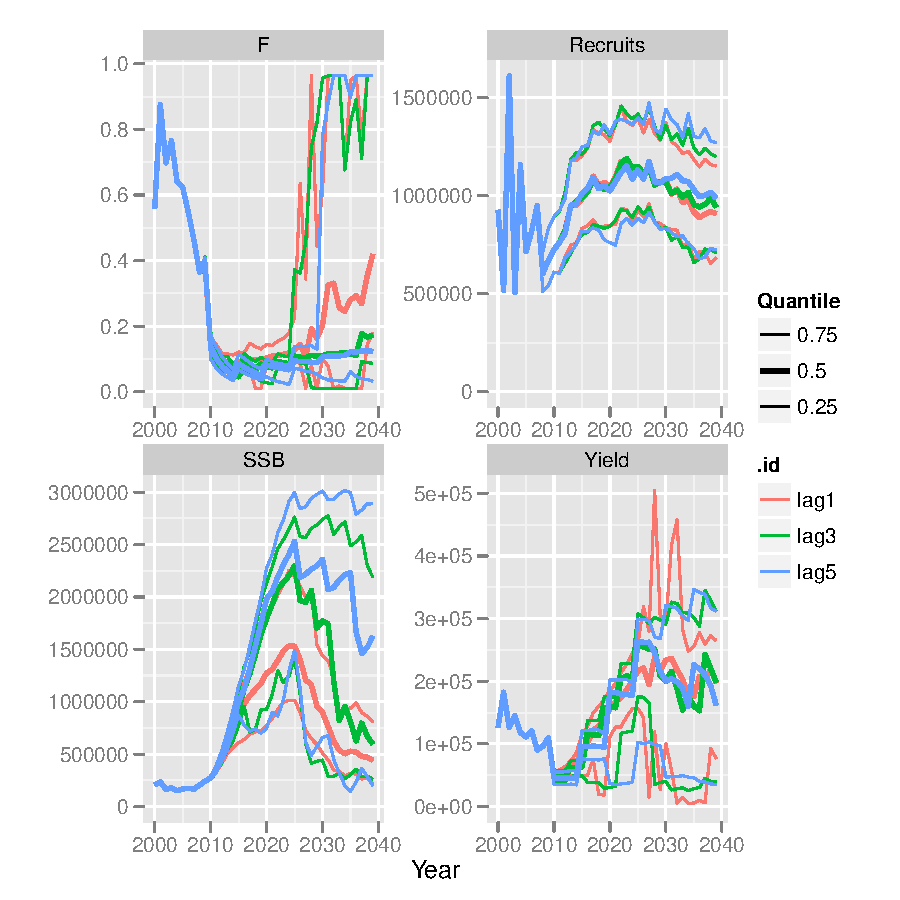
\includegraphics{MSE-004}
\caption{Projections with assessment lags of 1,3 and 5 years}
\label{fig:lags}
\end{figure}
 
\begin{figure}[H]
\centering
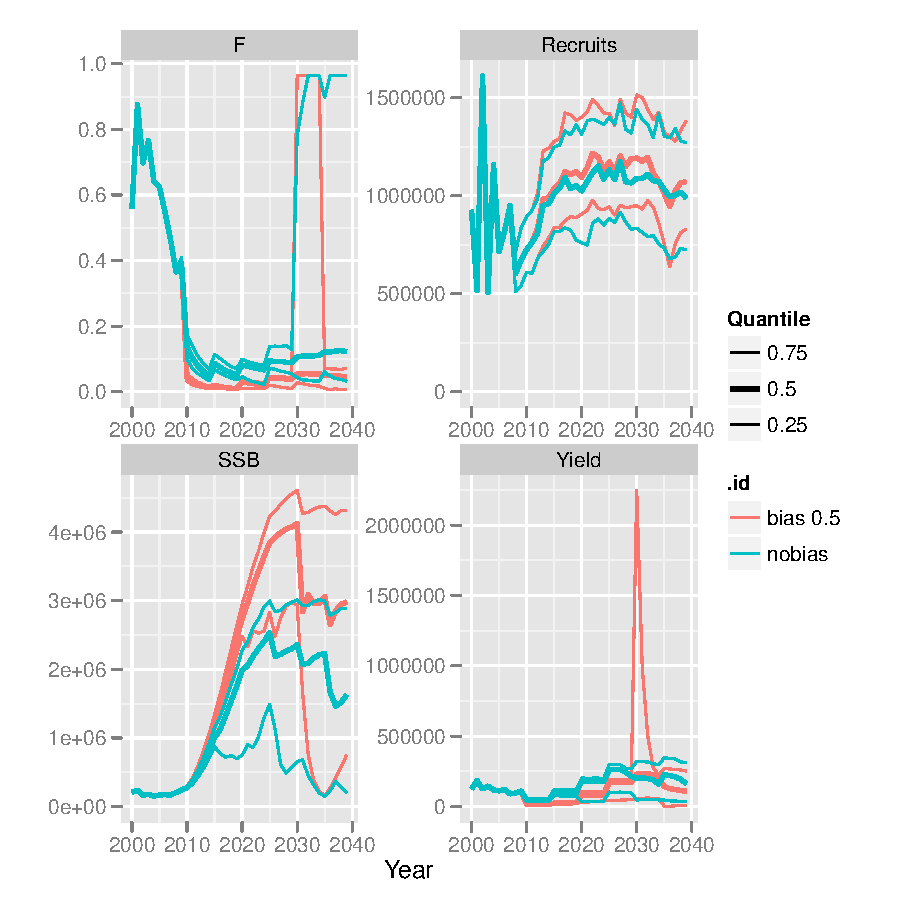
\includegraphics{MSE-005}
\caption{Projections with bias on the index of abundance}
\label{fig:srvBias}
\end{figure}

\begin{figure}[H]
\centering
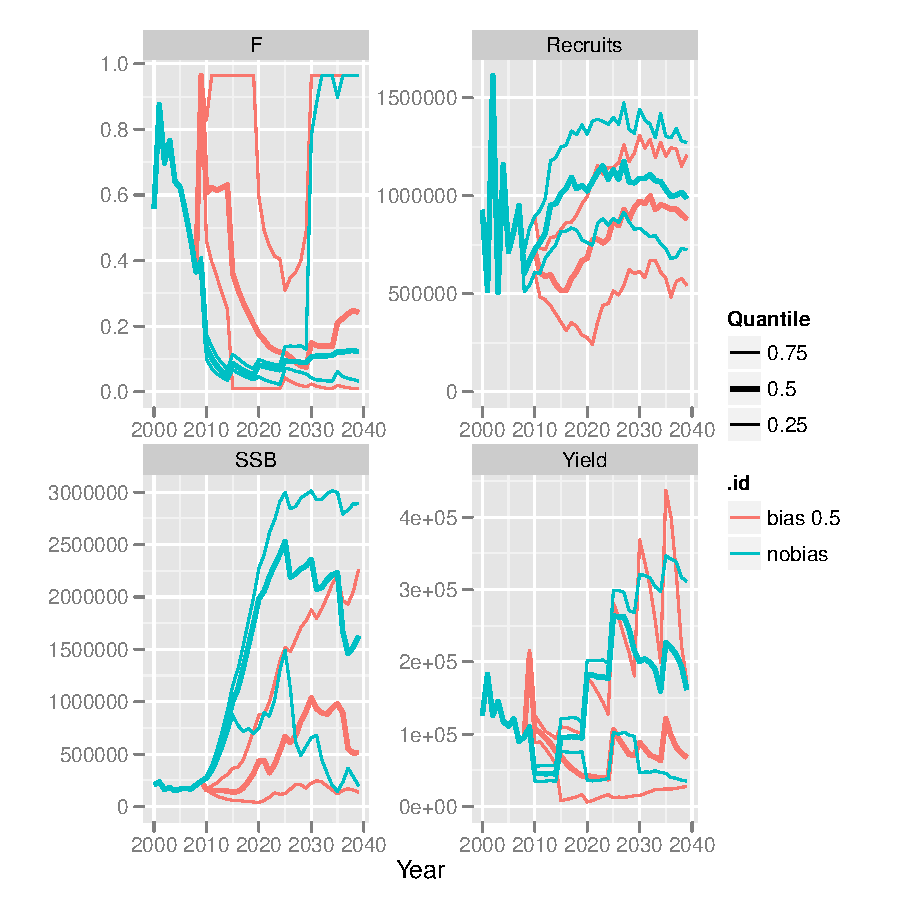
\includegraphics{MSE-006}
\caption{Projections with bias on catches}
\label{fig:cthBias}
\end{figure}

\begin{figure}[H]
\centering
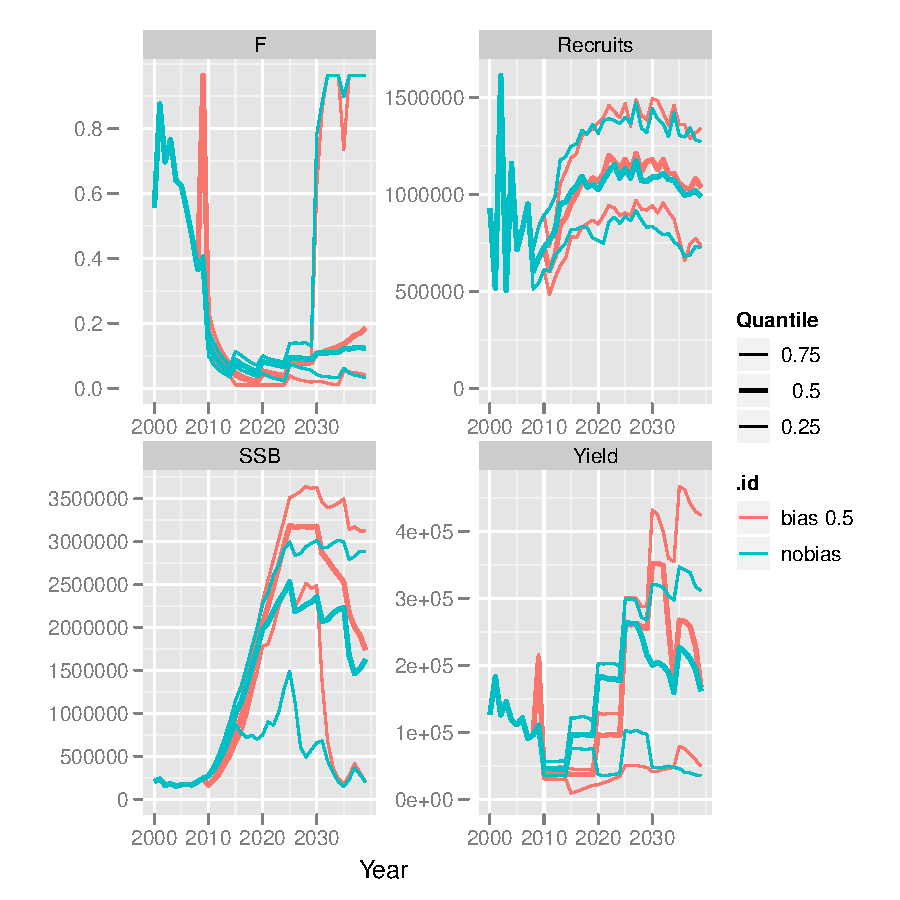
\includegraphics{MSE-007}
\caption{Projections with bias on catches and index}
\label{fig:2Bias}
\end{figure}

\end{document}

